\begin{UseCase}{CU 1.4.2}{Gestionar Proveedor} {
	
	El sistema muestra los proveedores a los que estamos afiliados y da acceso a los botones para buscar, agregar, eliminar y modificar de esos mismos.
}
	
\UCitem{Versión}{1.0}
\UCccsection{Administración}
\UCccitem{Autor}{Daniel Alexis Arroyo Ceja}
\UCccitem{Evaluador}{}
\UCccitem{Operación}{}
\UCccitem{Prioridad}{Media}
\UCccitem{Complejidad}{Baja}
\UCccitem{Volatilidad}{Baja}
\UCccitem{Madurez}{Alta}
\UCccitem{Estatus}{Finalizado}
\UCccitem{Fecha del último estatus}{20 de diciembre del 2021}

%% Copie y pegue este bloque tantas veces como revisiones tenga el caso de uso.
%% Esta sección la debe llenar solo el Revisor
% %--------------------------------------------------------
	%   % Revisión Versión (Anote la versión que se revisó.)
\UCccsection{Revisión Versión 0.1 }
% 	% FECHA: Anote la fecha en que se terminó la revisión.
\UCccitem{Fecha}{20 de diciembre del 2021} 
% 	% EVALUADOR: Coloque el nombre completo de quien realizó la revisión.
\UCccitem{Evaluador}{Josue Gonzaga}
% 	% RESULTADO: Coloque la palabra que mas se apegue al tipo de acción que el analista debe realizar.
\UCccitem{Resultado}{Cambios}
% 	% OBSERVACIONES: Liste los cambios que debe realizar el Analista.
\UCccitem{Observaciones}{
	\begin{UClist}
		\RCitem{PC1}{\DONE{Agregar diagramas, correcion de trayectoria principal }}{20 de diciembre del 2021}
	\end{UClist}		
}

% %--------------------------------------------------------
	
\UCsection{Atributos}
	\UCitem{Actor(es)}{
		\cdtRef{Actor:RT}{Empleado} 
	}
	\UCitem{Propósito}{
		Visualizar los proveedores afiliados a nuestra farmacia y buscar algun especifico en caso de necesitarse.
	}
	\UCitem{Entradas}{
		Nombre de la empresa
	}
	\UCitem{Salidas}{
		
		\begin{UClist}
			Información básica del proveedor.			
			\UCli  \cdtRef{Empleado:nombre}{Nombre}.
			
			\UCli \cdtRef{tesis:Título de la empresa}{Empresa}.
			
			\UCli \cdtRef{tesis:Telefono de contacto}{Telefono}.
			
			\UCli \cdtRef{tesis:Correo electronico}{Correo de contacto}.
		\end{UClist}
	}

	\UCitem{Precondiciones}{
		Haber proveedores ya registrados en la base de datos a partir de la opción “Agregar proveedor”.
	}
	\UCitem{Postcondiciones}{
		Ninguna
	}
	\UCitem{Reglas de negocio}{
		Ninguna
	}
	\UCitem{Errores}{
		-Que la base de datos no este disponible o este caida
		-Que no haya proveedores registrados
	}
	\UCitem{Tipo}{
		Ninguna
	}
\end{UseCase}

\begin{UCtrayectoria}
	
	\UCpaso [\UCactor]	Selecciona \cdtButton{Proveedores} en el la interfaz Menu principal. Consultar en página: \ref{UI: menu principal} 	

	\UCpaso [\UCsist]		Muestra la interfaz Gestionar proveedor.  \label{P2}

	\UCpaso [\UCsist]		Obtiene todos los datos de los proveedores de la BD. \refTray{A} \refTray{B}

	\UCpaso [\UCsist]		Muestra la interfaz Gestionar proveedor con los datos anteriores. Consultar en página: \ref{UI: gestionar proveedor} 

	\UCpaso[\UCactor] 		Ingresa el nombre de la empresa que desea encontrar en la barra de busqueda.
	
	\UCpaso[\UCactor]		Pulsa la opcion buscar.
	
	\UCpaso[\UCsist]		Busca coincidencias de lo que ingreso el usuario con los proveedores registrados en la base de datos. \refTray {B}

	\UCpaso[\UCsist]		Muestra los datos obtenidos al usuario. 
	
\end{UCtrayectoria}


%...........::::::::::::TRAYECTORIAS ALTERNATIVAS::::::::::::::........
%-------------------------Trayectoria A------------------------------
\begin{UCtrayectoriaA}{A}{El sistema no logra conectar con la base de datos.}
	
	\UCpaso[\UCsist] No logra obtener los datos de la base de datos
	
	\UCpaso[\UCsist] Muestra mensaje: No se logro conectar con la base de datos.
			
	\UCpaso[] Regresa a la interfaz principal.
	
\end{UCtrayectoriaA}

%-------------------------Trayectoria B------------------------------
\begin{UCtrayectoriaA}{B}{El sistema no logra encontrar al proveedor.}
	
	\UCpaso[\UCsist] Muestra mensaje: No se encontraron proveedores registrados con ese nombre.
			
	\UCpaso[] Regresa al paso 2 \ref{P2} de la trayectoria principal.
	
\end{UCtrayectoriaA}

{
\begin{flushleft}
	
	% Clases
	\Large{Clases}\\
	\rule{14cm}{0.5pt}

	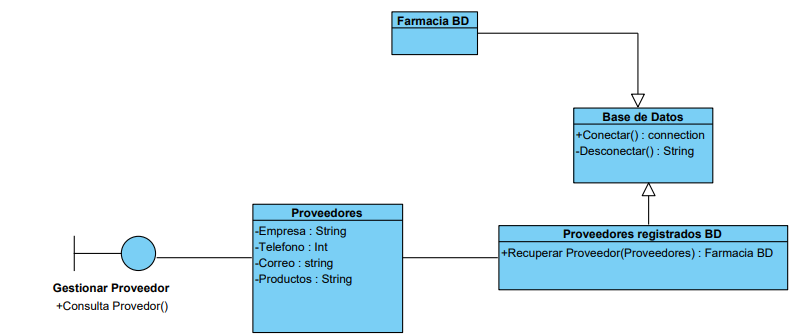
\includegraphics[width=14cm]{casouso/cu8/images/Diagrama de clases.jpg}\\	

	% Secuencia
	\Large{Secuencia}\\
	\rule{14cm}{0.5pt}

	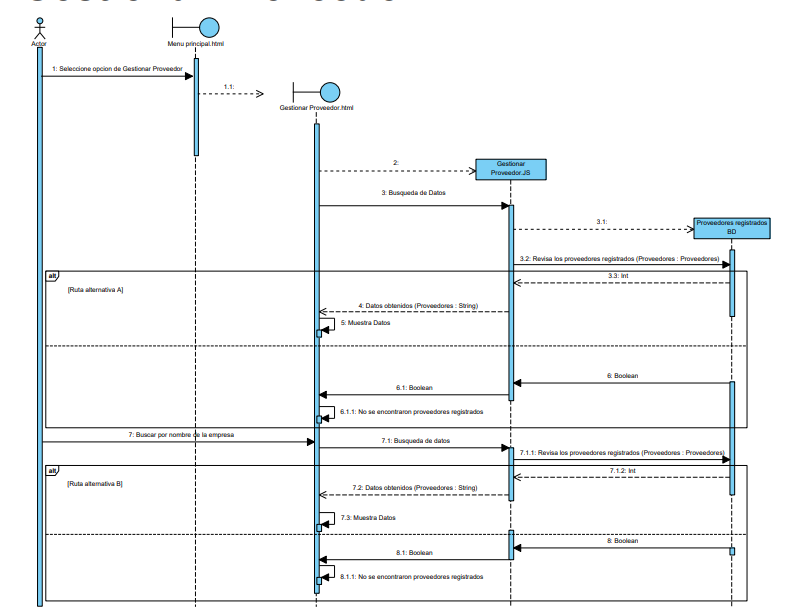
\includegraphics[width=14cm]{casouso/cu8/images/Diagrama secuencia.jpg}\\	
	
\end{flushleft}
}